\chapter{Konzeption der Anwendung}
\thispagestyle{fancy}

\section{Struktur der Anwendung}
In diesem Abschnitt soll zunächst die generelle Struktur der Anwendung definiert werden. Weite Teile der Struktur können dabei aus dem Praxisprojekt übernommen werden. Im Praxisprojekt wurden die folgenden Themengebiete behandelt:

\begin{itemize}
  \item Typographie
  \item Layout \& Struktur
  \item Whitespace
  \item Farben
  \item Bilder
  \item Interaktive Elemente
\end{itemize}

Nach einer erneuten evaluation der Ergebnisse des Praxisprojektes konnten die in der Abschlussarbeit zu behandelnden Themengebiete auf zunächst drei eingegrenzt werden (der Bereich \textit{Layout \& Struktur} wurde dabei in \textit{Layout \& Grids} umbenannt):

\begin{itemize}
  \item Typographie
  \item Layout \& Grids
  \item Farben
\end{itemize}

Diese Abgrenzung begründet sich auf verschiedene Weisen. Im Fall des Bereiches \textit{Whitespace} konnte im Rahmen des Praxisprojektes kein zufriedenstellendes Konzept erarbeitet werden, wodurch sich dieser Bereich per se nicht für eine Umsetzung eignet. Weiterhin muss es Ziel dieser Arbeit sein, am Schluss eine vollständige Anwendung zu erhalten. Um dieses Ziel im zeitlichen Rahmen erreichen zu können mussten weitere Themengebiete vernachlässigt werden. Hier boten sich die Bereiche \textit{Bilder} und \textit{Interaktive Elemente} an, da diese für die gestalterische Grundqualität eine vergleichsweise niedrige Rolle spielen. \textbf{NOTE: Vielleicht muss das hier noch belegt werden, wie ein Brötchen}. Diese Bereiche wurden aber ausreichend konzeptioniert und bieten sich als erste Erweiterungen für die Anwendung nach beenden der Arbeit an.

Außerdem müssen für die Anwendung jeweils ein nutzerfreundlicher Einstieg und Ausstieg gefunden werden. Diese wurden im Praxisprojekt nicht explizit ausgearbeitet und fallen somit auch Konzeptionell in den Bereich der Abschlussarbeit und werden später in diesem Kapitel behandelt.

Die finale Struktur der Anwendung für den Rahmen dieser Arbeit sieht also wie folgt aus:

\begin{itemize}
  \item Einstieg
  \item Typographie
  \item Layout \& Grids
  \item Farben
  \item Ausstieg
\end{itemize}

\section{Einstieg in die Anwendung}
Bereits im Praxisprojekt wurde festgestellt, dass es sinnvoll ist, das Zielmedium des Nutzers zu kennen. Mit Blick auf die Zielgruppe wurden hier drei mögliche Bereiche definiert: Native App, Website und Textdokument. \textbf{NOTE: Hier verweis auf Untersuchung im PP}. Diese Bereiche können jedoch auch in sich verschiedene Eigenarten aufweisen, so kann ein Textdokument beispielsweise für das Lesen an einem Bildschirm oder das Lesen in gedruckter Form entworfen werden. Eine komplette Auflistung der möglichen Bereiche oder \textit{scopes} der Anwendung findet sich in Abbildung \ref{fig:intro} auf Seite \pageref{fig:intro}.

\begin{figure}[h]
    \centering
    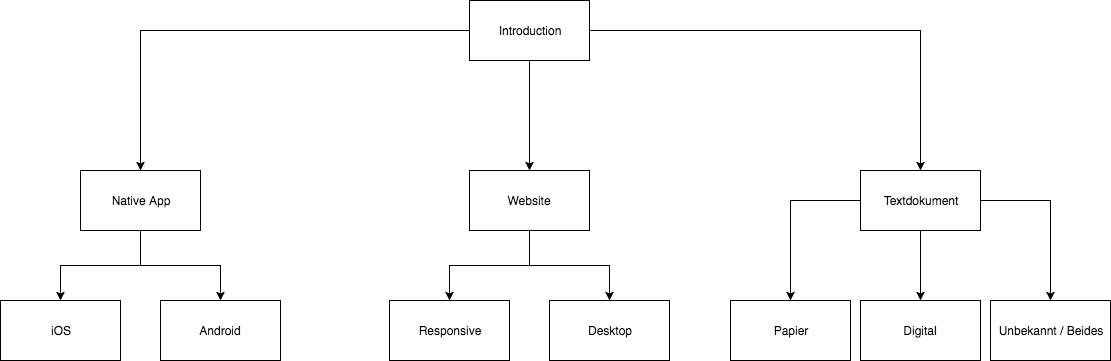
\includegraphics[width=1\textwidth]{images/ablauf_intro.png}
    \caption{Mögliche Entscheidungen im Einstieg der Anwendung}
    \label{fig:intro}
\end{figure}

Obwohl die Abgrenzung der Bereiche für die hier definierte Zielgruppe ausreichend ist, lassen sich bereits jetzt einige Stellen erkennen, die bei einer möglichen späteren Erweiterung der Zielgruppe überarbeitet werden müsste. Vorrangig betrifft das den Bereich \textit{Website}. Hier ist die vorhandene Unterteilung in \textit{Responnsive} und \textit{Desktop} für ein Echtwelt-Szenario unter Umständen zu allgemein gehalten.

Um den kognitiven Aufwand \textbf{Beleg} für den Nutzer möglichst gering zu halten, bietet es sich an, ihn Schrittweise durch das Festlegen des für ihn passenden Bereiches zu führen.

\section{Typographie}

\section{Farben}

\section{Layouts \& Grid}


\section{Ergebnisse der Benutzung}
Eines der Ziele der Anwendung ist es, dem Nutzer währen der Nutzung auf interaktive weise Wissen zu vermitteln. Da der Nutzer jedoch während der Nutzung auch konkrete Ergebnisse erarbeitet wäre es hier kontraproduktiv, ihm diese Ergebnisse nicht am Ende der Anwendung noch einmal explizit zukommen zu lassen (zusätzlich zum implizit gesammelten Wissen).

Dieser Bereich wurde im Rahmen des Praxisprojektes nicht ausdefiniert, ist aber für die Wahrnehmung der Anwendung als fertiges Produkt durchaus wichtig. Eine gute Darstellung der Ergebnisse des Nutzers definieren einen ausschlaggebenden Teil der Nutzungserfahrung.
Hier sollen also mögliche Darstellungen der Ergebnisse diskutiert werden und vorrangig zwei Fragen beantwortet werden:
\begin{enumerate}
  \item Welche Darstellung der Ergebnisse ist für den Nutzer am Vorteilhaftesten?
  \item Welche Darstellung bietet den besten Kompromiss aus Umsetzbarkeit und Mehrwert für den Nutzer?
\end{enumerate}

Die einfachste Darstellung ist eine Transistente Darstellung innerhalb der Anwendung am Ende der Verwendung. Eine Darstellung ist wegen der Haltung der ermittelten Werte im Redux-Store der Anwendung einfach. Obwohl einfach umzusetzen, ist diese Lösung nicht optimal: Nachdem der Nutzer die Anwendung schließt sind die erarbeiteten Daten verloren, da diese nicht persistent gespeichert werden.

Ein naheliegender Schritt ist also eine Persitierung des Wissens für den Nutzer. Hier bieten sich verschiedene Möglichkeiten, wie zum Beispiel das Speichern in Cookies oder das Entwicklen eines Backends, an. Ein Kompromiss zwischen Usability und Entwicklungsaufwand wäre hierbei die persistieren des Wissen in einer herunterladbarer Datei, beispielsweise als PDF.

Eine weitere Frage beschäftigt sich mit dem Aufbau dieser Datei. Auch hier wäre der einfachste Ansatz, die Ergebnisse des Nutzers einfach aufzulisten. Optimal wäre eine Aufbereitung der Daten, sodass der Nutzer diese möglichst ohne weitere Manipulation in seinen Workflow übernehmen kann. Obwohl das Zielmedium des Nutzers bekannt ist, zeigt sich hier das Problem, dass innerhalb dieser Zielmedien weiterhin verschieden Tools verwendet werden können, die eine unterschiedliche Aufbereitung der Daten erfordern.
Beispielsweise kann bekannt sein, dass der Nutzer eine Webandwendung entwickelt und das Styling für seine texte in CSS vornimmt. Trotzdem kann der Nutzer zum Beispiel verschieden Preprozessoren wie SCSS, SASS oder LESS verwenden, die alle eine unterschiedliche Syntax verwenden.
Es liegt dabei durchaus im Rahmen des Möglichen, diese Informationen vom Nutzer zu erhalten und die Daten entsprechend aufzubereiten, jedoch liegen diese Anforderungen außerhalb des Zeitlichen Rahmens dieser Abschlussarbeit.

Hier wird dem Nutzer daher zunächst eine PDF zur Verfügung gestellt. Ein exemplarischer Aufbau kann ABB. XYZ entnommen werden.
